%\documentclass[spanish]{ijsra}
\def\IJSRAidentifier{\currfilebase} %<---- don’t change this!
%-------Title | Email | Keywords | Abstract-------------
\def\shorttitle{8th World Archaeology Congress 2016}
\def\maintitle{Giving the Past a Future: Review of the 8th World Archaeology Congress 2016 – {28th} August – {2nd} September Kyoto, Japan}
\def\cmail{rhaw9263@uni.sydney.edu.au}%, mcmaster.francesca@gmail.com}
%\def\keywords{Review, annual meeting, 8th}
%\def\keywordname{}%<--- redefine the name “Keywords“ in needed language
%\def\abstract{}
%--------Author’s names------------
\def\authorone{Rebekah Hawkins}
\def\authortwo{Francesca McMaster}
%-------Biographical information-------------
\def\bioone{Rebekah Hawkins graduated last year with a Bachelor of Arts majoring in archaeology and a Bachelor of Science majoring in Anatomy and Geology from the University of Sydney. Next year she will start her honours year focusing on the analysis of lithic artefacts from Lake George in NSW, Australia. She was the president of the Sydney University Archaeology Society, Chair of the Organising Committee for the National Archaeology Student Conference Australia 2015 and is currently a Student Representative for the Australia Archaeology Association. She took this year off to hike the length of Nepal across the Himalayas and looks forward to starting her own research next year and continuing to represent archaeology students across Australia.}

\def\biotwo{Francesca McMaster recently graduated from the University of Sydney with first class honours in archaeology and a bachelor of arts in archaeology and art history. Her thesis research focused on the application of ethnography in Indigenous Australian archaeological interpretation. Her general research interests include the role of archaeology in the formation of concepts of nationalism and identity, including but not limited to, the use of analogy within archaeological interpretation and the continuing influence of colonisation in archaeology. Francesca currently works for museums and archaeological consultancies in Sydney, Australia. }
%------University/Institution--------------
\def\affilone{Department of Archaeology, The University of Sydney, Australia}


\begin{filecontents}{\IJSRAidentifier.bib}
@misc{closingWAC,
	title = {Closing Comments to WAC-8 and announcement of the creation of the Joan Gero Book Award},
	url = {http://worldarch.org/blog/closing-comments-to-wac-8-and-announcement-of-the-creation-of-the-joan-gero-book-award/},
	journal = {World Archaeological Congress News},
	publisher = {World Archaeological Congress},
	year = {2016},
	month = {Sept}
}

@misc{addressWAC,
	title = {Presidents Address at WAC-8},
	url = {http://worldarch.org/blog/presidents-address-at-wac-8/},
	journal = {World Archaeological Congress News},
	publisher = {World Archaeological Congress},
	year = {2016},
	month = {Sept}
}

@misc{aboutWAC,
	title = {WAC, About WAC},
	url = {http://worldarch.org/about-wac/},
	journal = {World Archaeological Congress News},
	publisher = {World Archaeological Congress},
	year = {2016},
	month = {Sept}
}

@misc{welcomeWAC,
	title = {Welcome to WAC-8 Kyoto},
	url = {http://wac8.org/},
	journal = {World Archaeological Congress News},
	publisher = {World Archaeological Congress},
	year = {2016},
	month = {Sept}
}
\end{filecontents}

%\begin{document}
%\begin{otherlanguage}{spanish}
\IJSRAopening
%-------
\lettrine{T}{he} The World Archaeological Congress was founded 30 years ago to develop a global forum for archaeological conversation. As stated on WAC’s website, the congress meets to promote:
\begin{itemize}
	\item the exchange of results from archaeological research;
	\item professional training and public education for disadvantaged nations, groups and communities;
	\item the empowerment and support of Indigenous groups and First Nations peoples;
	\item and the conservation of archaeological sites \parencite{aboutWAC}.
\end{itemize}

WAC-8 was \IJSRAsection{WAC-8}held from August \nth{28} to September \nth{2} 2016 in the historic city of Kyoto, Japan. Easily accessible, Kyoto is a major Japanese city connected to both Osaka and Tokyo airports by \textit{Shinkansen} (bullet train). Historically important, Kyoto was the long serving capital of Imperial Japan before the capital moved to Tokyo in 1869. Now a bustling modern city, Kyoto provides the perfect backdrop for an archaeological conference, melding the modern with ancient tradition. The green hills surrounding the modern urban center hide a plethora of cultural and historical sites, not to mention the rich variety of Japanese cuisine available throughout the city. For the discipline of archaeology in Japan, Kyoto is also an important historic site. As Hiroshi Tsude, Chair of WAC-8 Kyoto Local Organising Committee notes, one hundred years ago Dr Kosaku Hamada founded academic archaeology, as the first archaeology professor, at Kyoto University \parencite{welcomeWAC}. 

The many tours that were on offer to conference attendees showcased these cultural sites, both in Kyoto and in surrounding regions, with both day trips and multi-day trips. These excursions included sites such as the world’s oldest wooden building the Horyuji Temple in Nara, the sake brewery museum and Nijo Castle (see Figs \ref{fig:Hawkins-Figure01}, \ref{fig:Hawkins-Figure02}, \& \ref{fig:Hawkins-Figure03}). One post-conference tour even took delegates to Japan’s northern island Hokkaido on a two-night/three-day tour focusing on the Indigenous Ainu culture and associated prehistoric sites.

\begin{figure}[!htb] %Figure 1
	\centering
	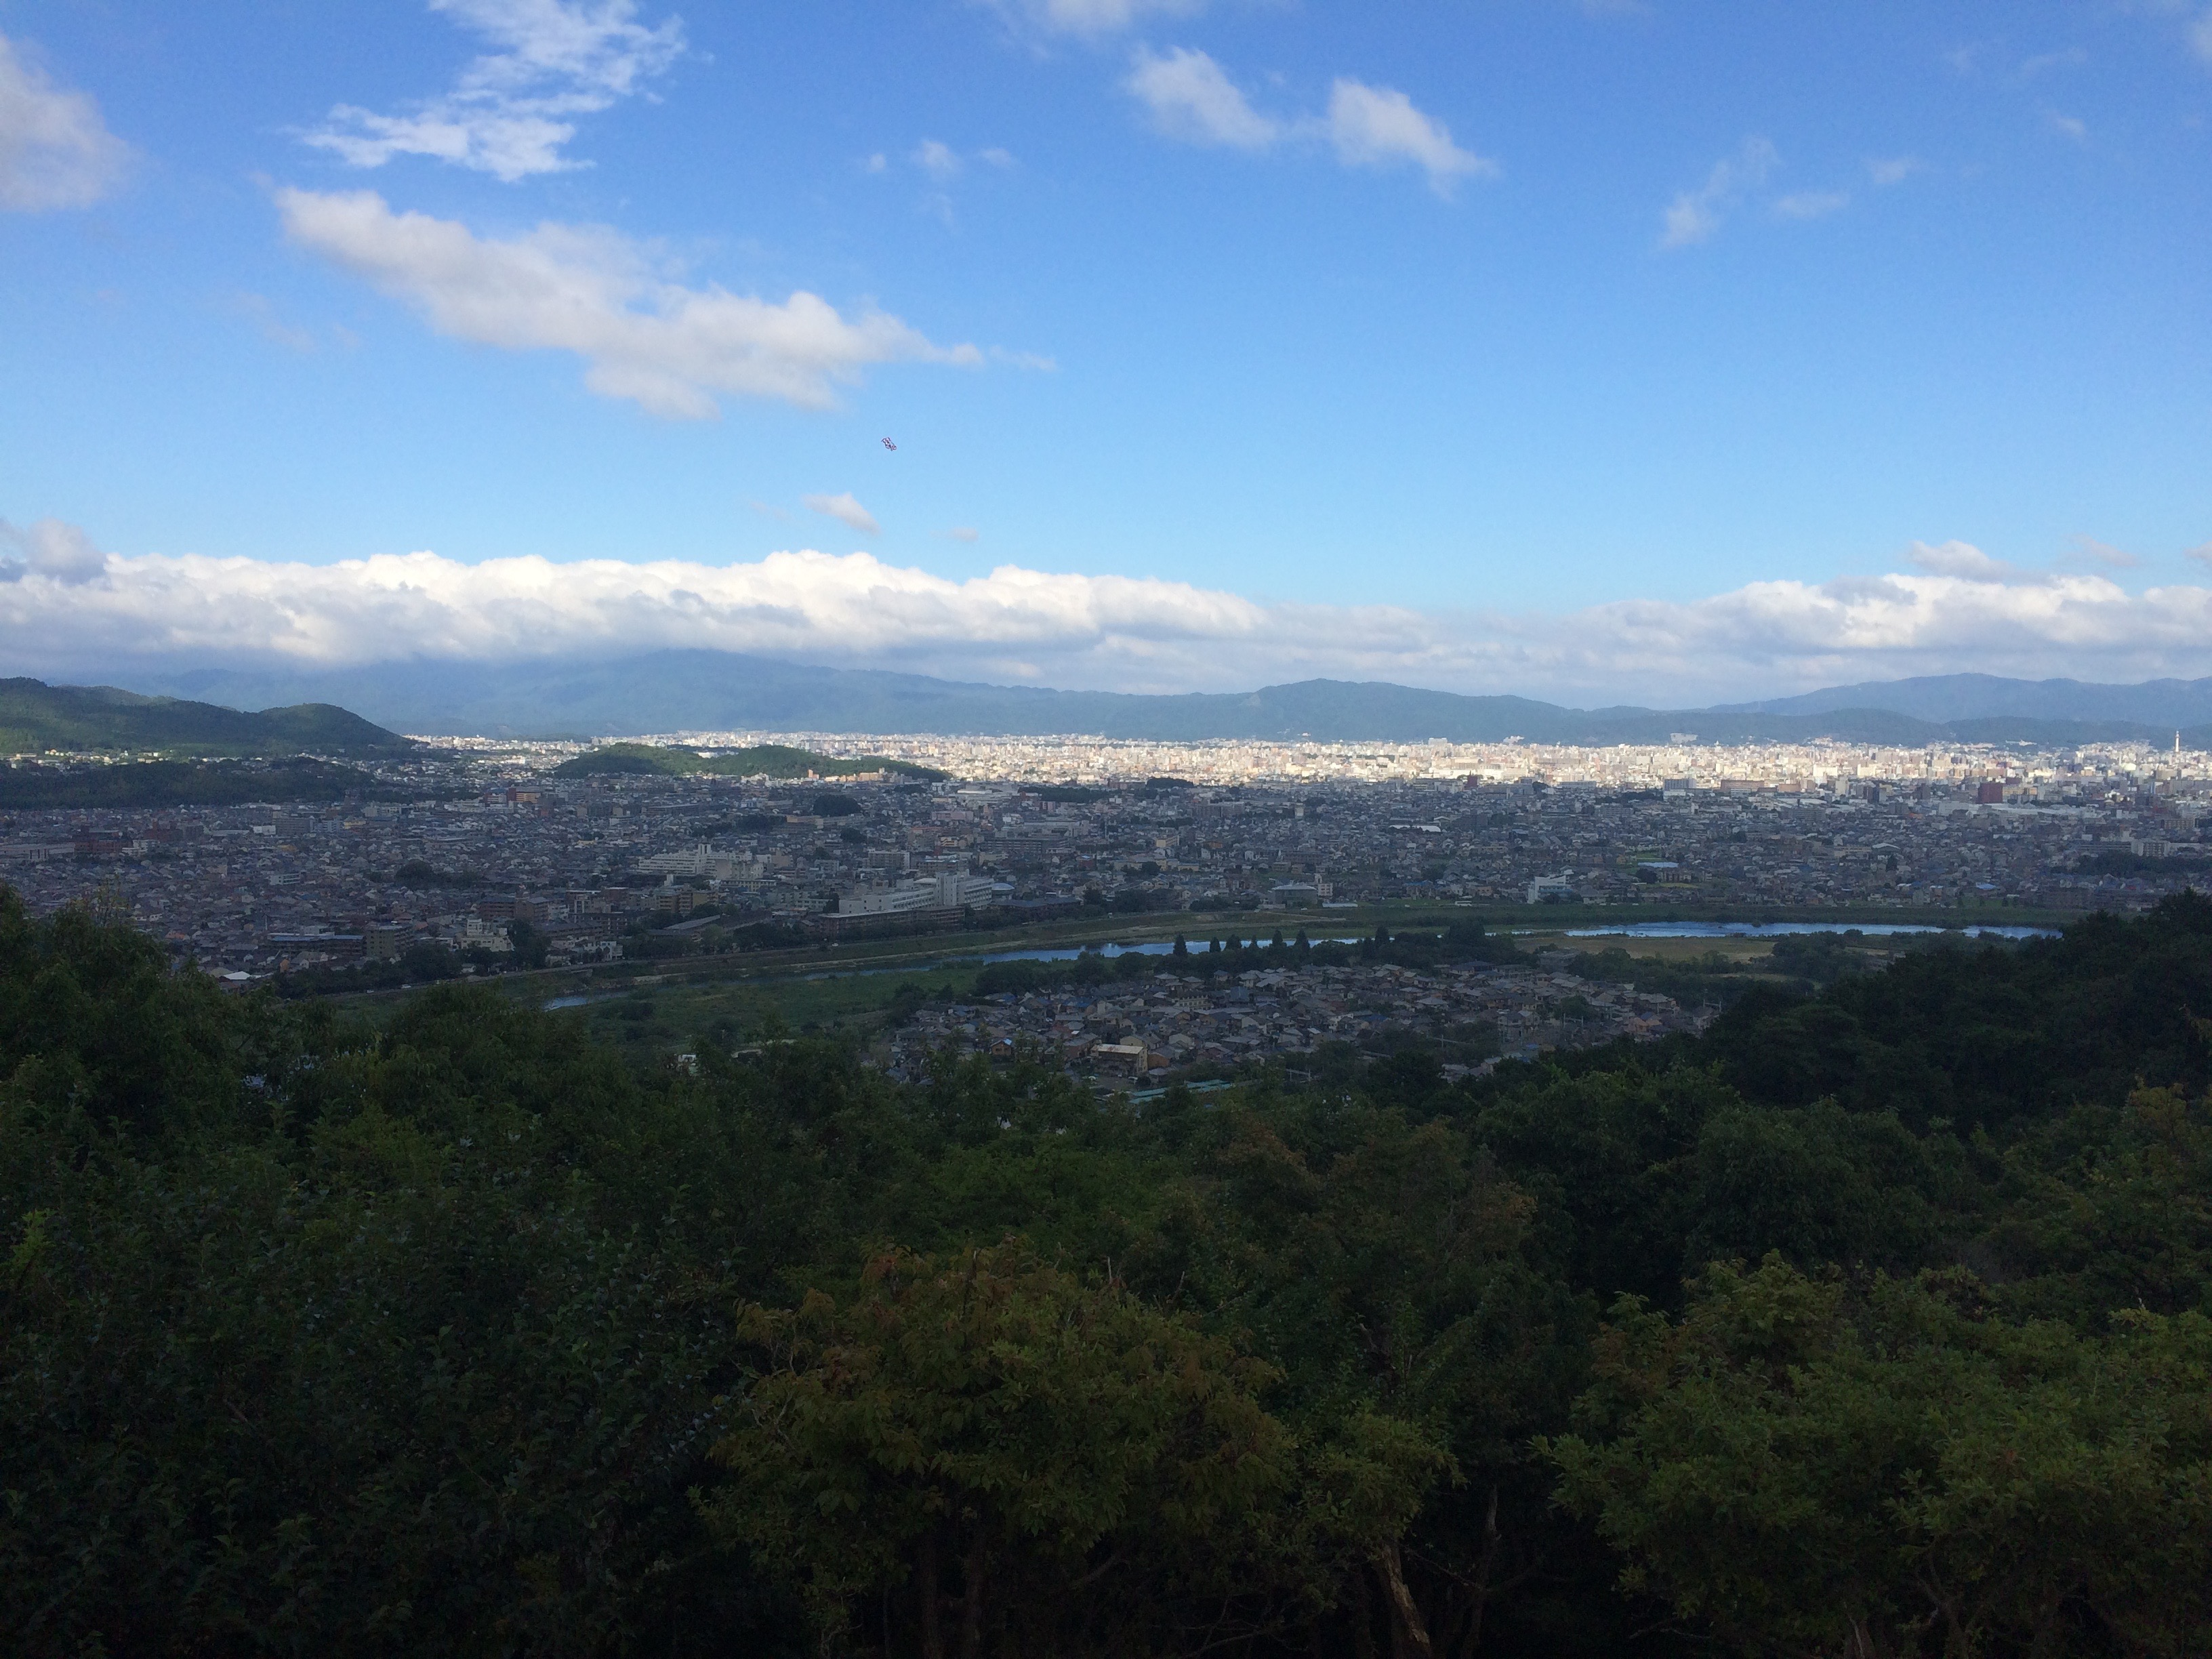
\includegraphics[width=\linewidth]{Hawkins-Figure01}
	\caption{Sites around Kyoto: Looking over Kyoto from Arashiyama.  
		{\normalfont\scriptsize \\ \copyright\ by Matt Taylor 2016}}
	\label{fig:Hawkins-Figure01}
\end{figure}

\begin{figure}[!htb] %Figure 2
	\centering
	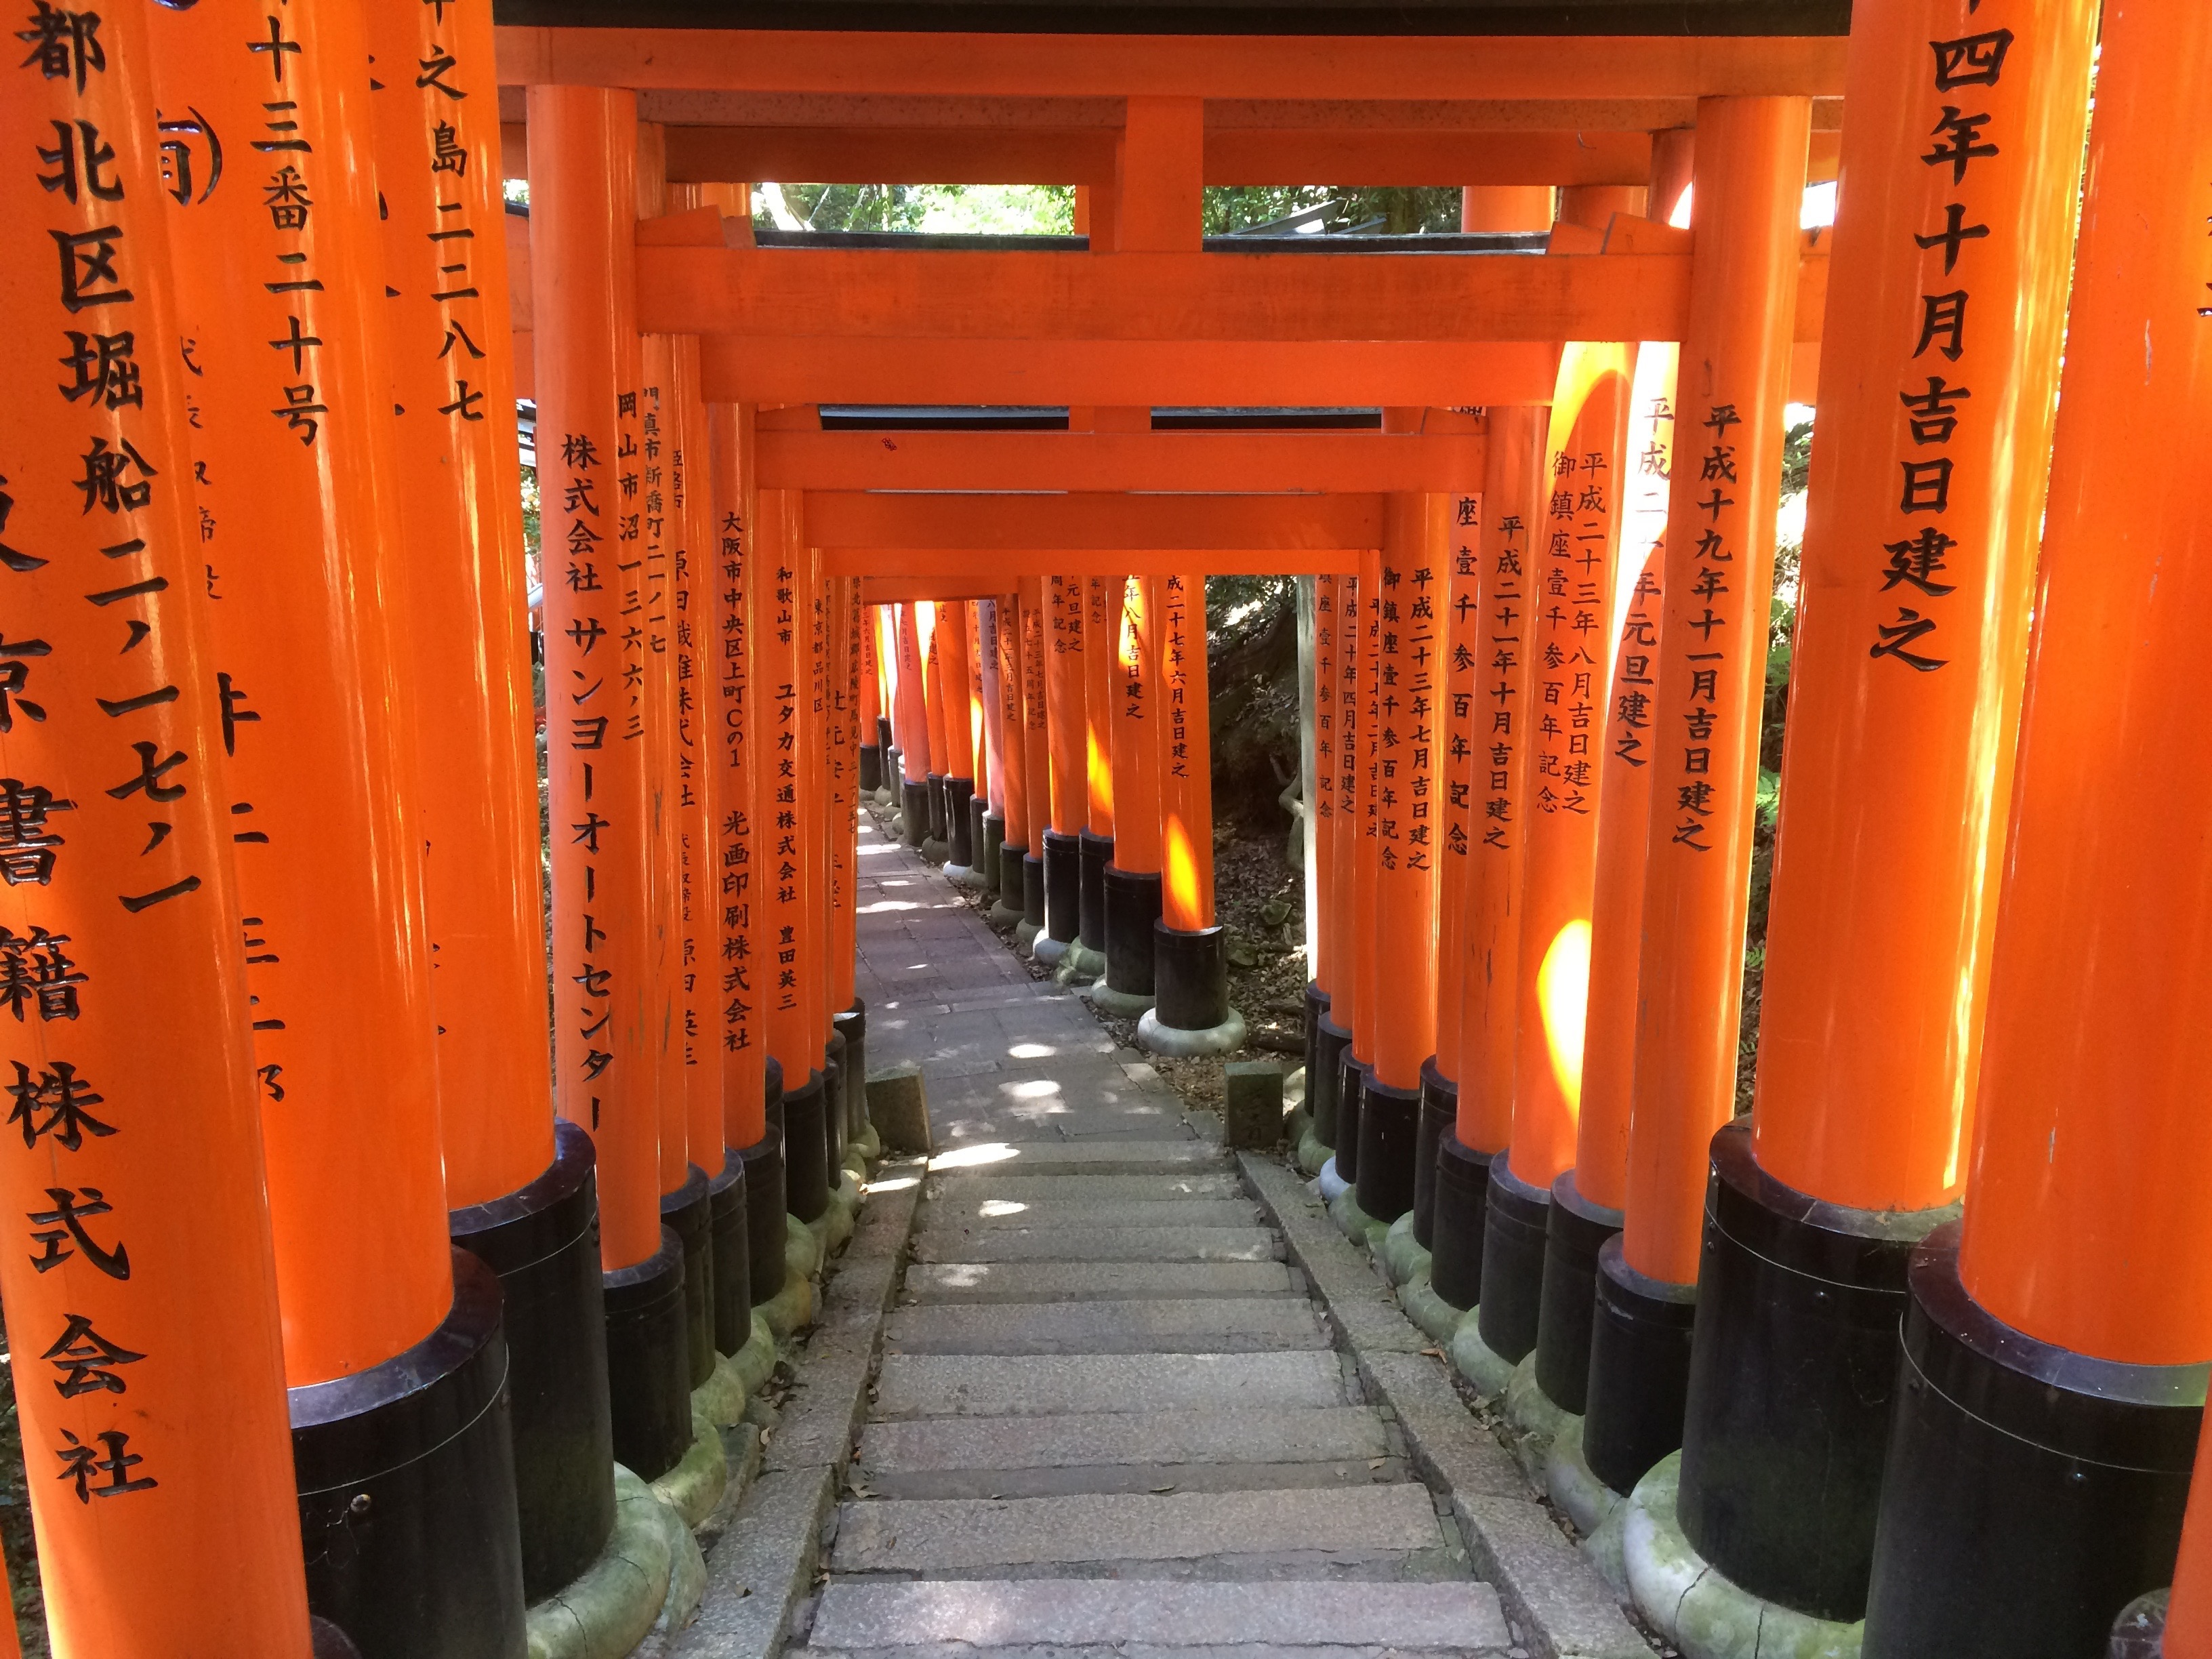
\includegraphics[width=\linewidth]{Hawkins-Figure02}
	\caption{Sites around Kyoto: Fushimi-inari temple in Kyoto. 
		{\normalfont\scriptsize \\ \copyright\ by Matt Taylor 2016}}
	\label{fig:Hawkins-Figure02}
\end{figure}

\begin{figure}[!htb] %Figure 3
	\centering
	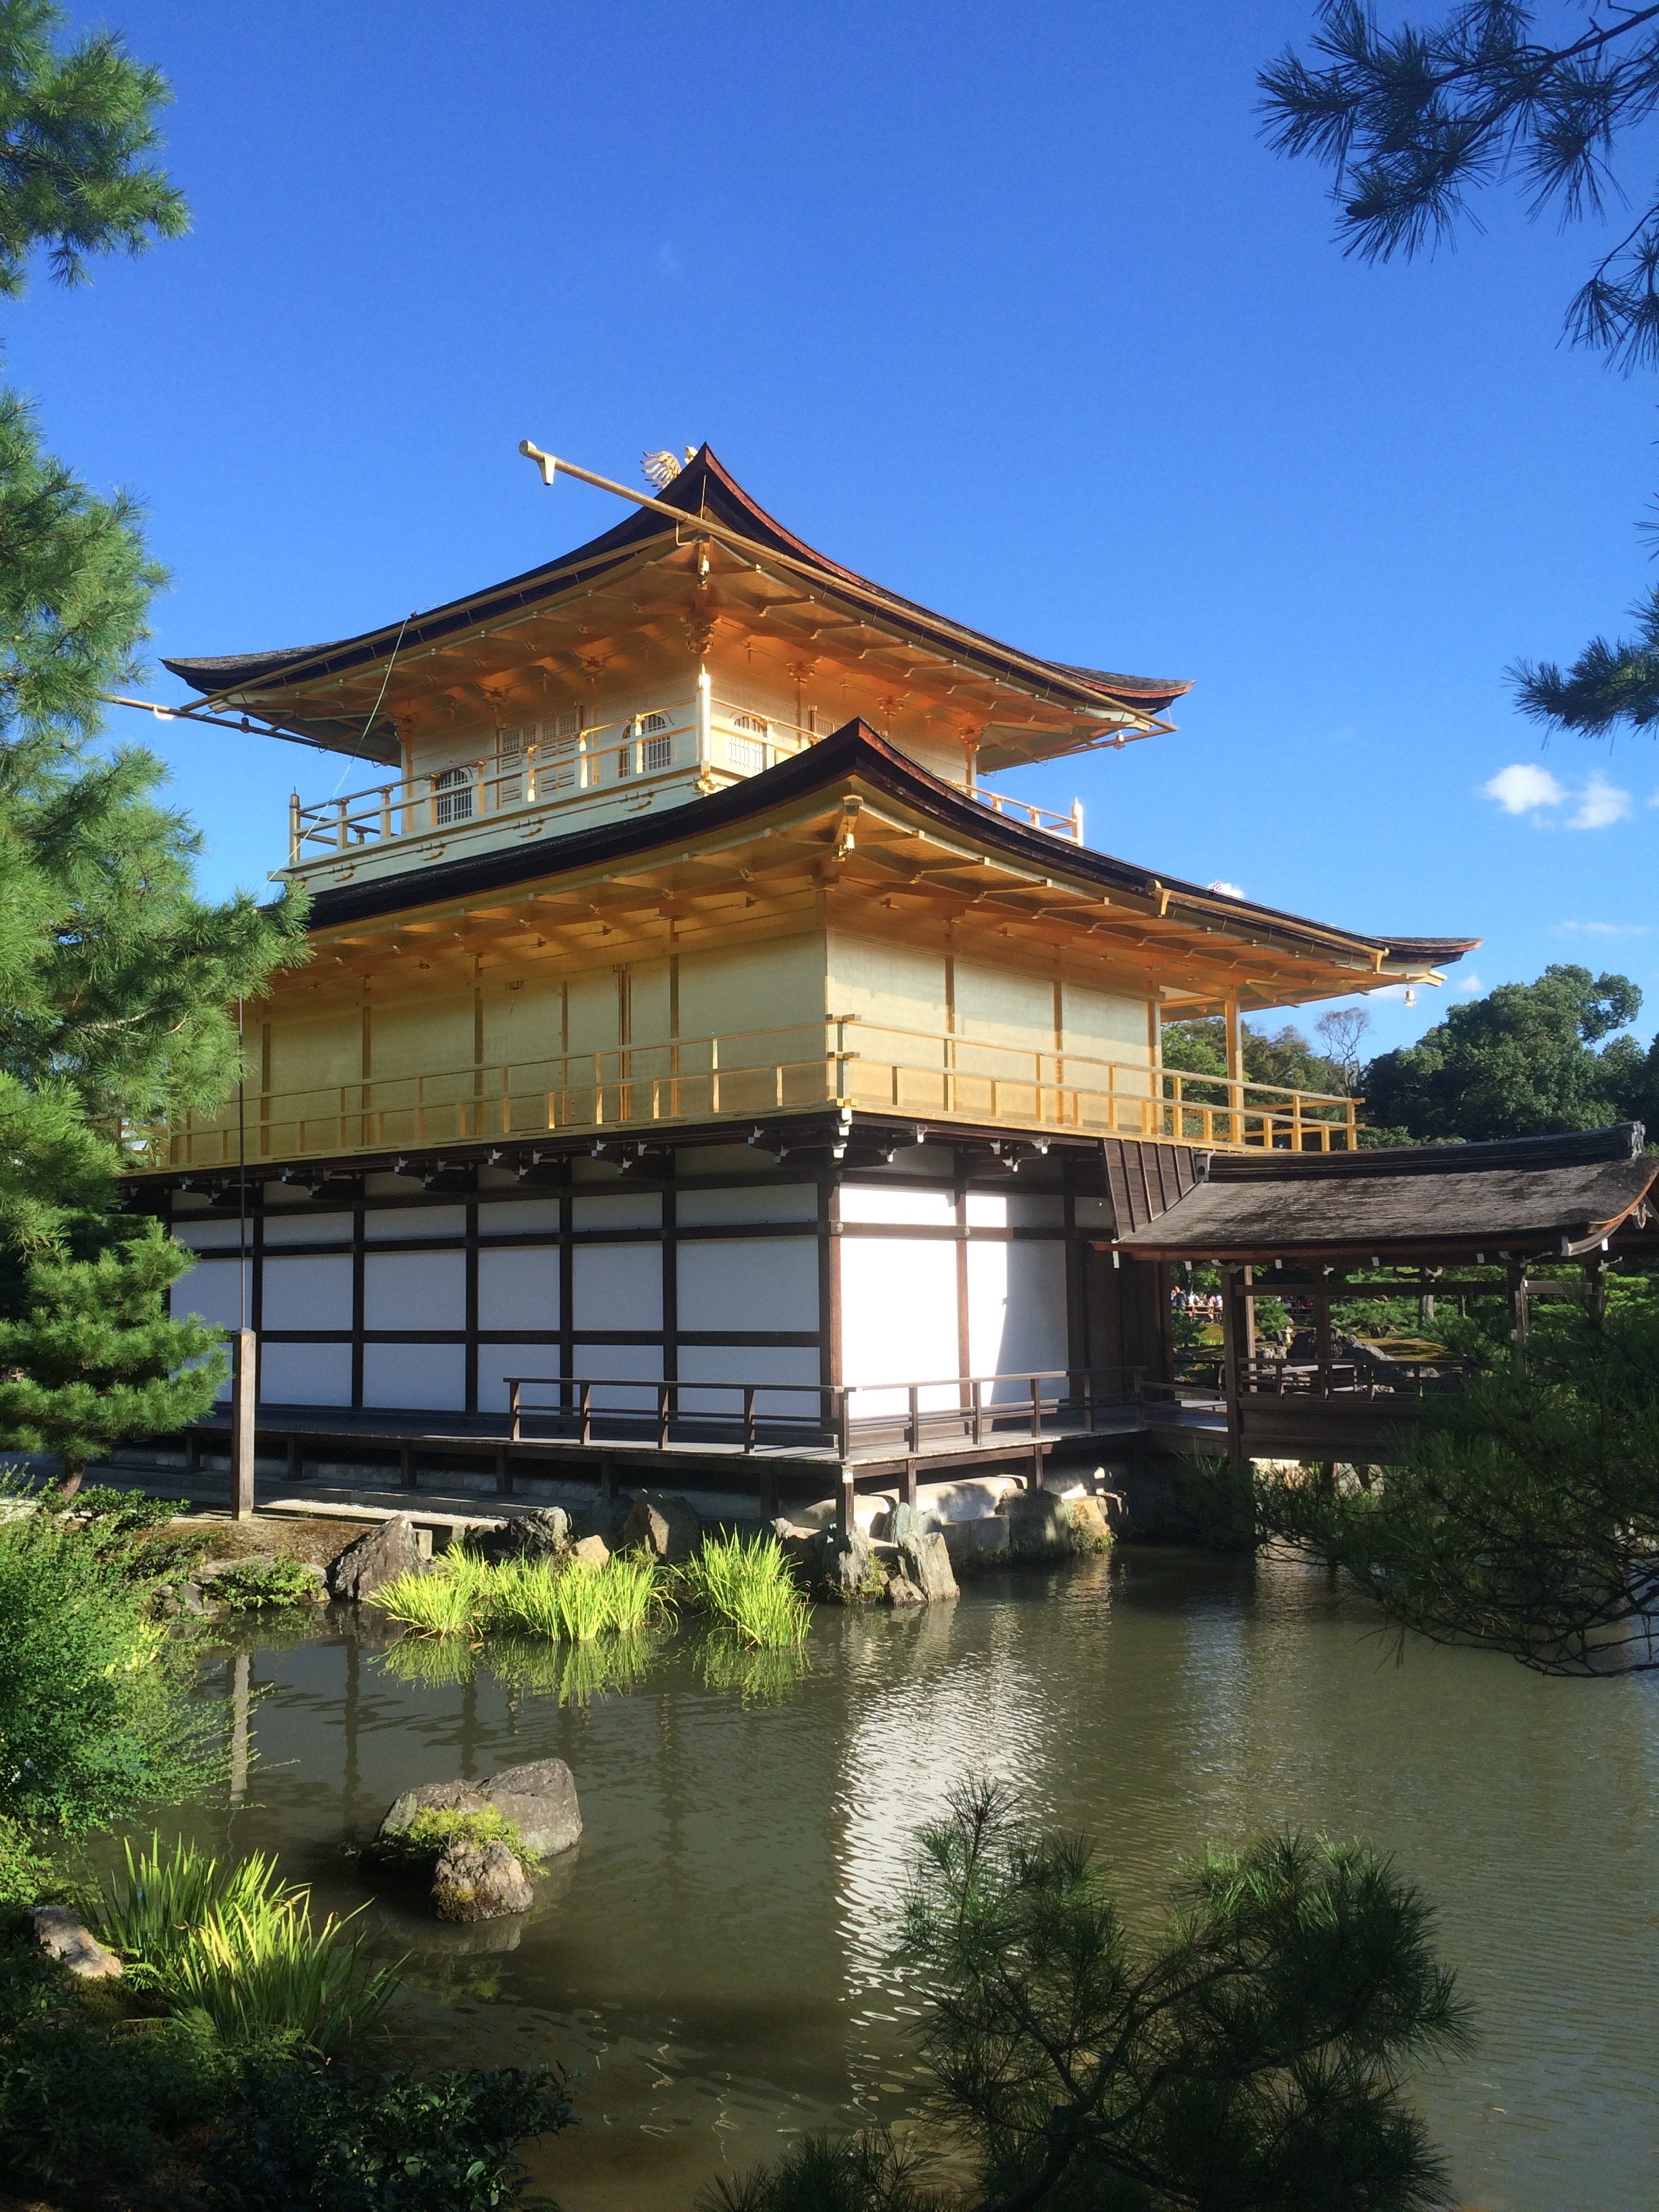
\includegraphics[width=\linewidth]{Hawkins-Figure03}
	\caption{Sites around Kyoto: The Golden Pavilion in Kyoto. 
		{\normalfont\scriptsize \\ \copyright\ by Matt Taylor 2016}}
	\label{fig:Hawkins-Figure03}
\end{figure}
  
WAC-8 was held at the centrally located Doshisha University, utilising their numerous lecture and tutorial rooms, cafeteria, auditorium and other facilities. Doshisha University proved the perfect space for a large conference of this kind to take place, where sessions, plenaries and public symposiums could be run and morning tea, lunch and afternoon tea served. The local organising committee did an astounding job to facilitate this conference, with an army of friendly student volunteers wearing easy to spot orange t-shirts on hand to assist in the day-to-day running of the conference. 

Registration opened \IJSRAsection{Opening ceremony highlights}on Sunday the 28th August at Doshisha University. Volunteers welcomed attendees and handed out all of the usual conference paraphernalia including a presentation guide of over \num{400} pages, giving a sense of the immense number of papers to be presented at the conference. At the Opening Ceremony attendees were offered translation devices in either Japanese or English as the speeches were given in both languages. This was a well thought out and appreciated gesture and a step towards overcoming the language barrier that President Koji Mizoguchi would go on to mention. 

In his welcoming address WAC President Koji Mizoguchi emphasised the immense amount of time and effort the organising committee had gone to make WAC-8 possible. In particular he outlined the many barriers that non-English speaking people face when they have to convey their message in English, noting that it erodes their sense of security and identity. This was an extremely relevant comment in relation to the location of the conference and the many international attendees from non-English speaking backgrounds. President Mizoguchi made a powerful statement when he reminded the audience that archaeology is not in the singular, but rather it is a conglomeration of hundreds of social settings, histories, cultures and identities. He went on to request WAC attendees set aside their differences and aim for the creation of, what he described as, an “ideal speech situation”, where information and opinions are exchanged between people of different social, cultural, political, historical and economic backgrounds \parencite{addressWAC}. It was an emotive and inspiring speech that emphasised the importance of WAC as an international organisation, particularly in light of current global crises that threaten not only global heritage, but also the stability of modern cultures \footnote{To listen to President Mizoguchi’s inspiring speech visit the \href{http://worldarch.org/blog/presidents-address-at-wac-8/}{WAC website}.}.

Professor Claire Smith, the previous WAC President, made a brave and well-received speech in Japanese, providing the English translation as she spoke. It was a meaningful act that truly highlighted the language barriers at international conferences, especially for native English speakers who do not often have to consider this obstacle. 

Subsequently a number of speakers gave the audience an overview of the 100-year history of Japanese archaeology, and as students who had never studied Japanese archaeology, this was a very useful and relevant introduction. Of particular interest was the Indigenous archaeology talk by Hirofumi Kato. Kato’s talk outlined the many issues still faced by the Indigenous Ainu peoples of Japan, who were only recognised in 2008. The opening day concluded with a reception held at Doshisha University where new and old acquaintances were met.

What struck \IJSRAsection{Overview of sessions}a lot of attendees was the number of parallel sessions run each day. In general there were 25 sessions running at the same time making it very difficult for people to choose what they wanted to see and what they would have to miss out on. There was an amazing range of sessions from Zooarchaeology, to the archaeology of Kyoto, to ideas of Entanglement, there really was something for everyone. Attending specific talks was difficult as schedules for some sessions changed making it near impossible to work out the exact time that certain speakers would present.

\begin{figure}[!htb] %Figure 4
	\centering
	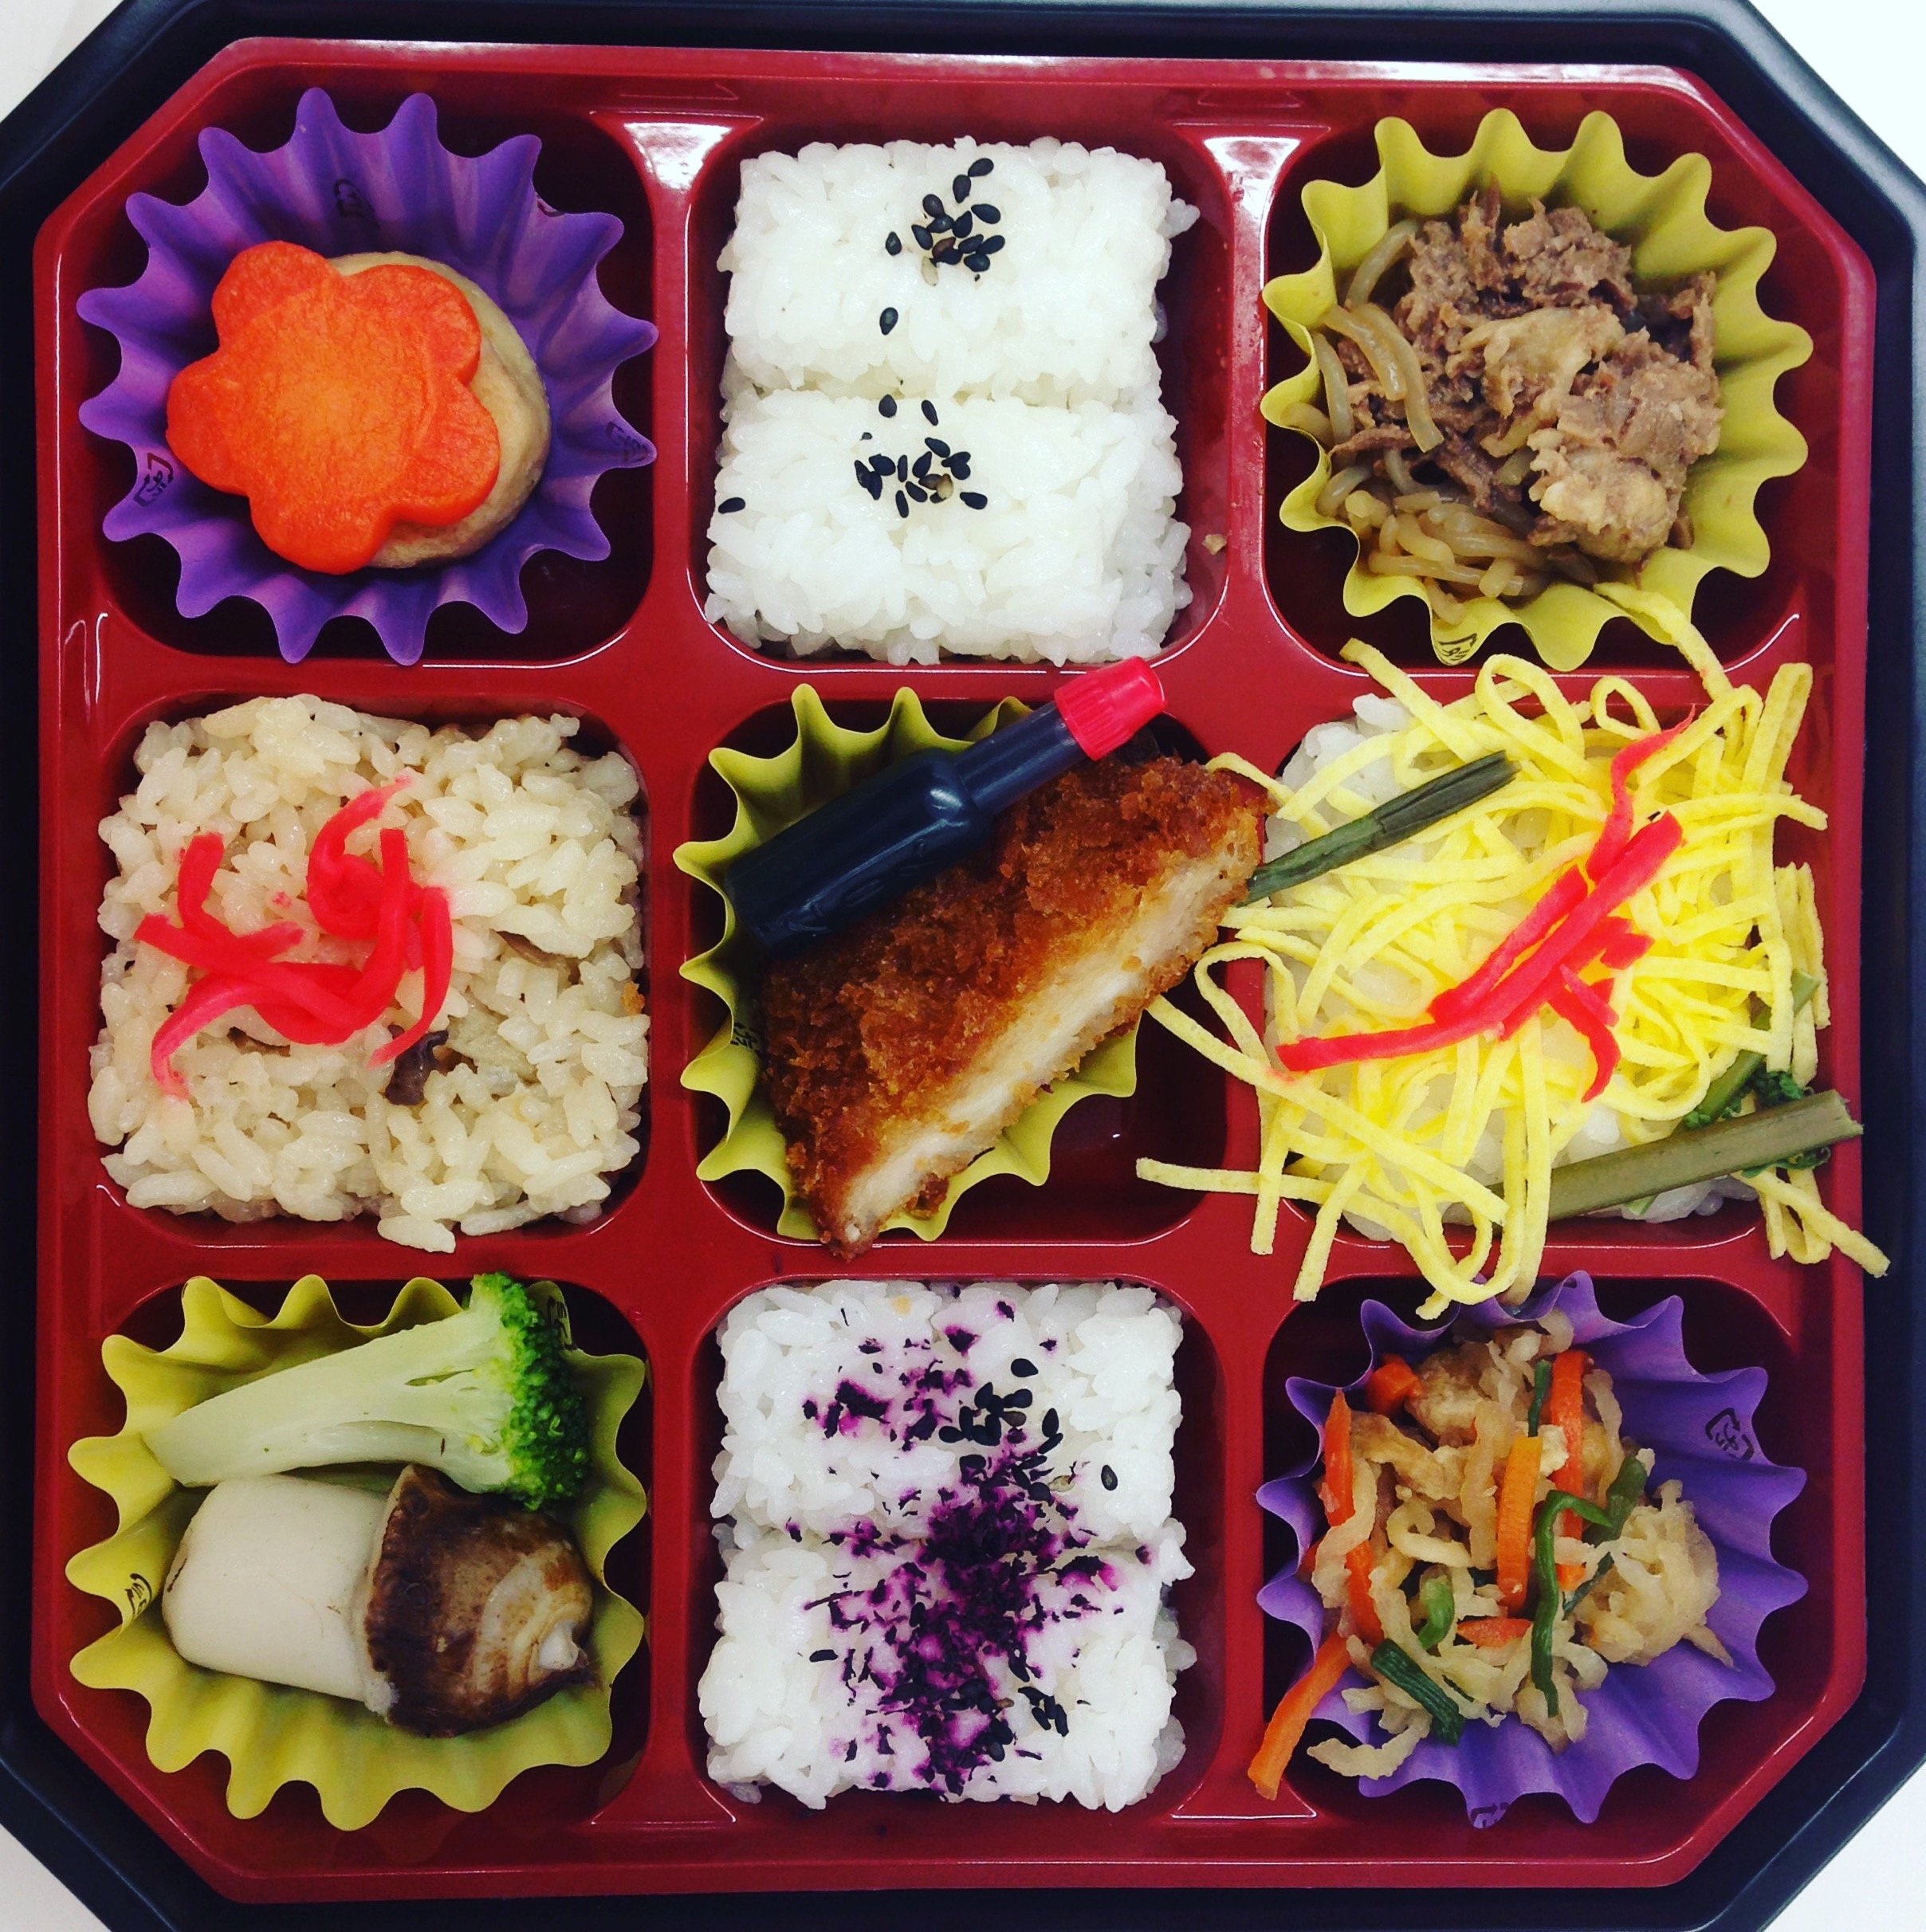
\includegraphics[width=\linewidth]{Hawkins-Figure04}
	\caption{Bento Box lunch provided by WAC-8. 
		{\normalfont\scriptsize \\ \copyright\ by \authortwo 2016}}
	\label{fig:Hawkins-Figure04}
\end{figure}

However, despite these challenges there was a great array of speakers in many of the sessions, with a large Japanese cohort in certain sessions and plenty of postgraduate and undergraduate speakers alongside professional archaeologists and academics. The language barrier posed its difficulties but all speakers showed perseverance and determination to overcome the obstacle. On Monday the first plenary was given called ‘\textit{Give the Past a Future}’ and that night the public symposium focused on world heritage sites in modern cities. 

The following day the Peter Ucko Memorial lecture was given by Peter Schmidt who also won the Peter Ucko prize, a very deserving awardee whose focus over the past number of decades on the decolonisation of archaeology in Africa has had major positive outcomes. That afternoon, of particular interest to students, was the WAC Student Committee Forum on Careers in International Heritage. Marta Lorenzon and Kate Ellenberger, both members of the WAC Student Committee, ran this session. There were four panellists for the forum, Hilary Soderland, Naima Benkari, John Carman and Jane Baxter, with each panellist bringing their own specific speciality to the discussion. The session was determined by what the students wanted to ask the panel with Marta and Kate facilitating the discussion. Questions from students queries such as: How did you get to where you are? Do you recommend specialising in a certain area? And how important is volunteering? The main advice that was given was that there is no right or wrong path to a career in archaeology with the importance of gathering transferrable skills stressed by all four panellists. Such skills can lead to archaeological careers in a diverse range of areas, such as academia, government, NGO’s or in the private sector. Heavy emphasis was placed on the importance of volunteer work, networking and ensuring that you are following a path that you enjoy. 

On Tuesday night the final Public Symposium was given on ‘\textit{Disaster Prevention and Archaeology}’ a very relevant topic of discussion in light of Japan’s unstable geology. Talks ranged from volcanic destruction and nuclear disasters, to tsunamis and their impacts and everlasting effect on communities around the world.

On Wednesday there was a mid-conference break to allow participants to enjoy the sites and tastes of Kyoto. 

Thursday saw the plenary, ‘\textit{Indigenous Archaeologies and World Archaeological Congress, the Past, the Present and the Future}’. This plenary was an informative and inclusive session, bringing together Indigenous archaeologists from around the globe to give their outlook on local issues affecting their cultures. Although giving very different perspectives from around the world, all five speakers highlighted a general message stating the ongoing lack of national and international recognition for Indigenous peoples. The convener of the plenary, Uzma Z. Rizvi, encouraged questions and statements from Indigenous audience members following the presentations to allow even more perspectives and concerns to be raised, before opening the discussion to all attendants. Statements and suggestions from the audience were noted to contribute to a statement on the future of Indigenous archaeology and WAC.  

Day 5 of the conference also offered WAC-8 participants the opportunity to visit an open archaeological site at the Kyoto Prefectural office, walking distance from Doshisha University. The Kyoto Prefectural office site offered an insight for archaeologists from around the world to see urban archaeology taking place in Kyoto and to hear from Japanese archaeologists the methods being used and the discoveries being made. Thursday ended with the WAC-8 Gala dinner, held at Kyoto Brighton Hotel (Figs \ref{fig:Hawkins-Figure05} \& \ref{fig:Hawkins-Figure06}). 

\begin{figure}[!htb] %Figure 5
	\centering
	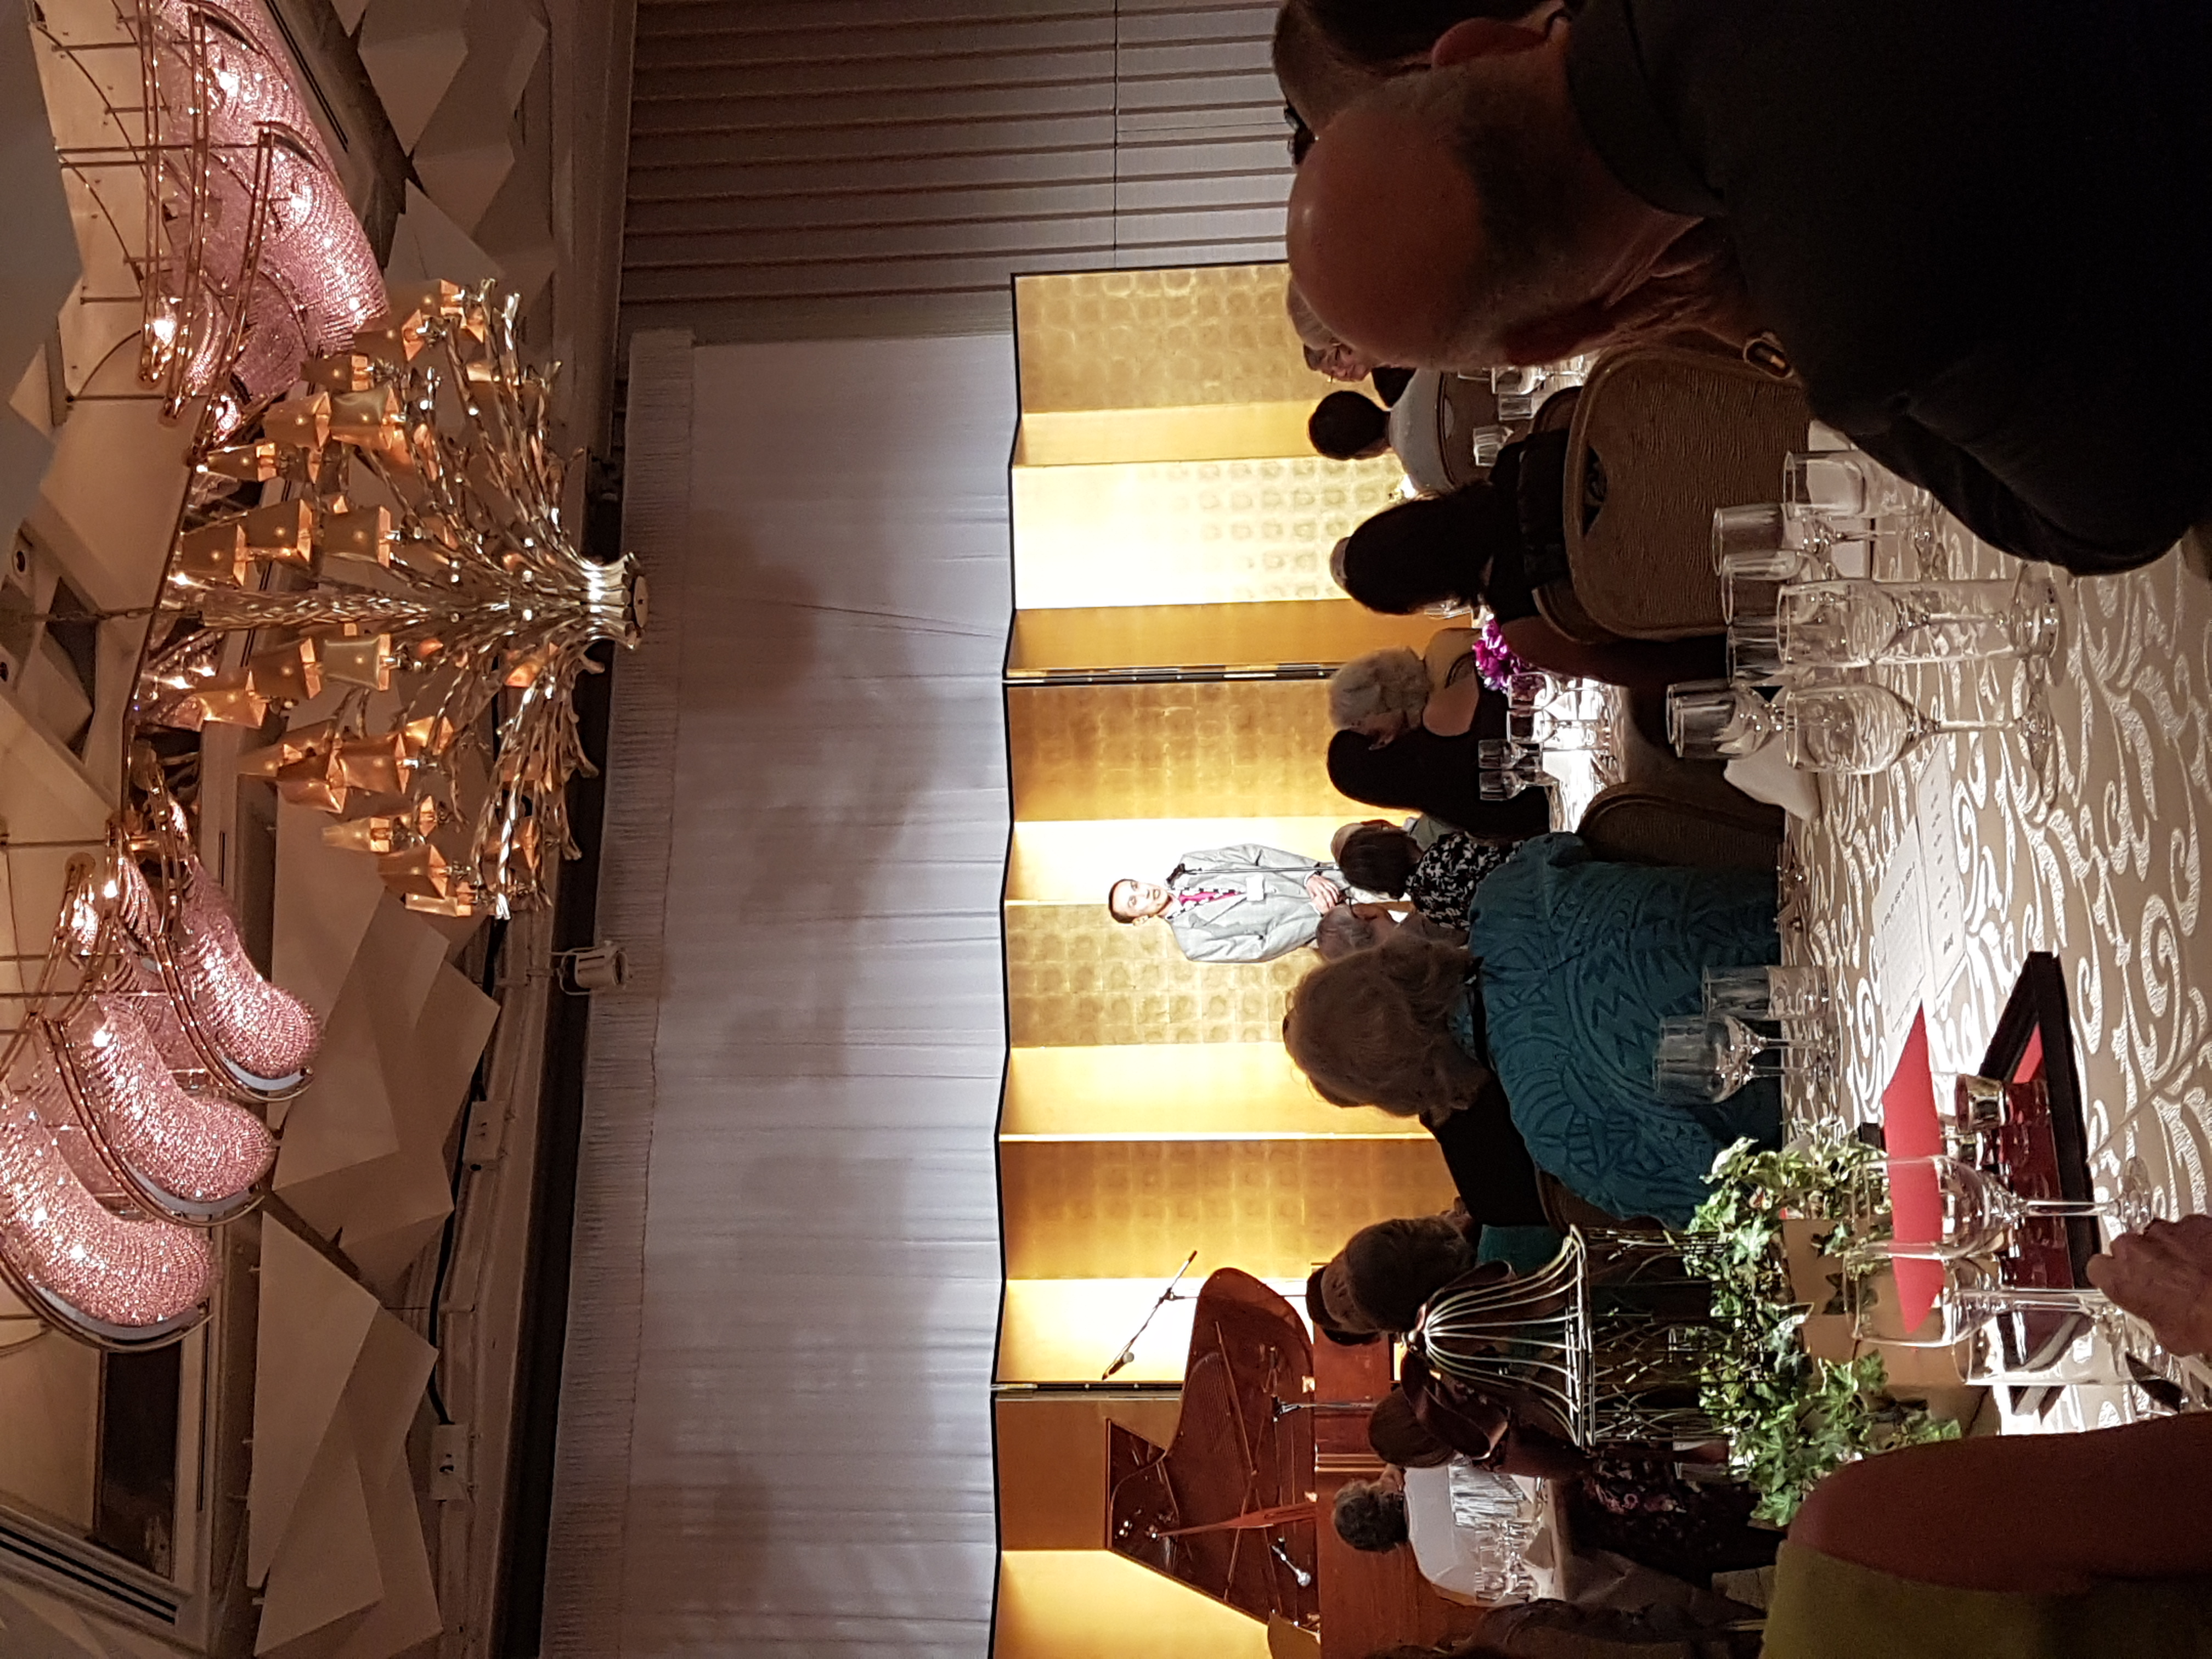
\includegraphics[width=\linewidth,angle=270]{Hawkins-Figure05}
	\caption{President Kohi Mizoguichi addressing the Gala Dinner at Kyoto Brighton Hotel. 
		{\normalfont\scriptsize \\ \copyright\ by Antoinette Hennessy 2016}}
	\label{fig:Hawkins-Figure05}
\end{figure}

\begin{figure}[!htb] %Figure 6
	\centering
	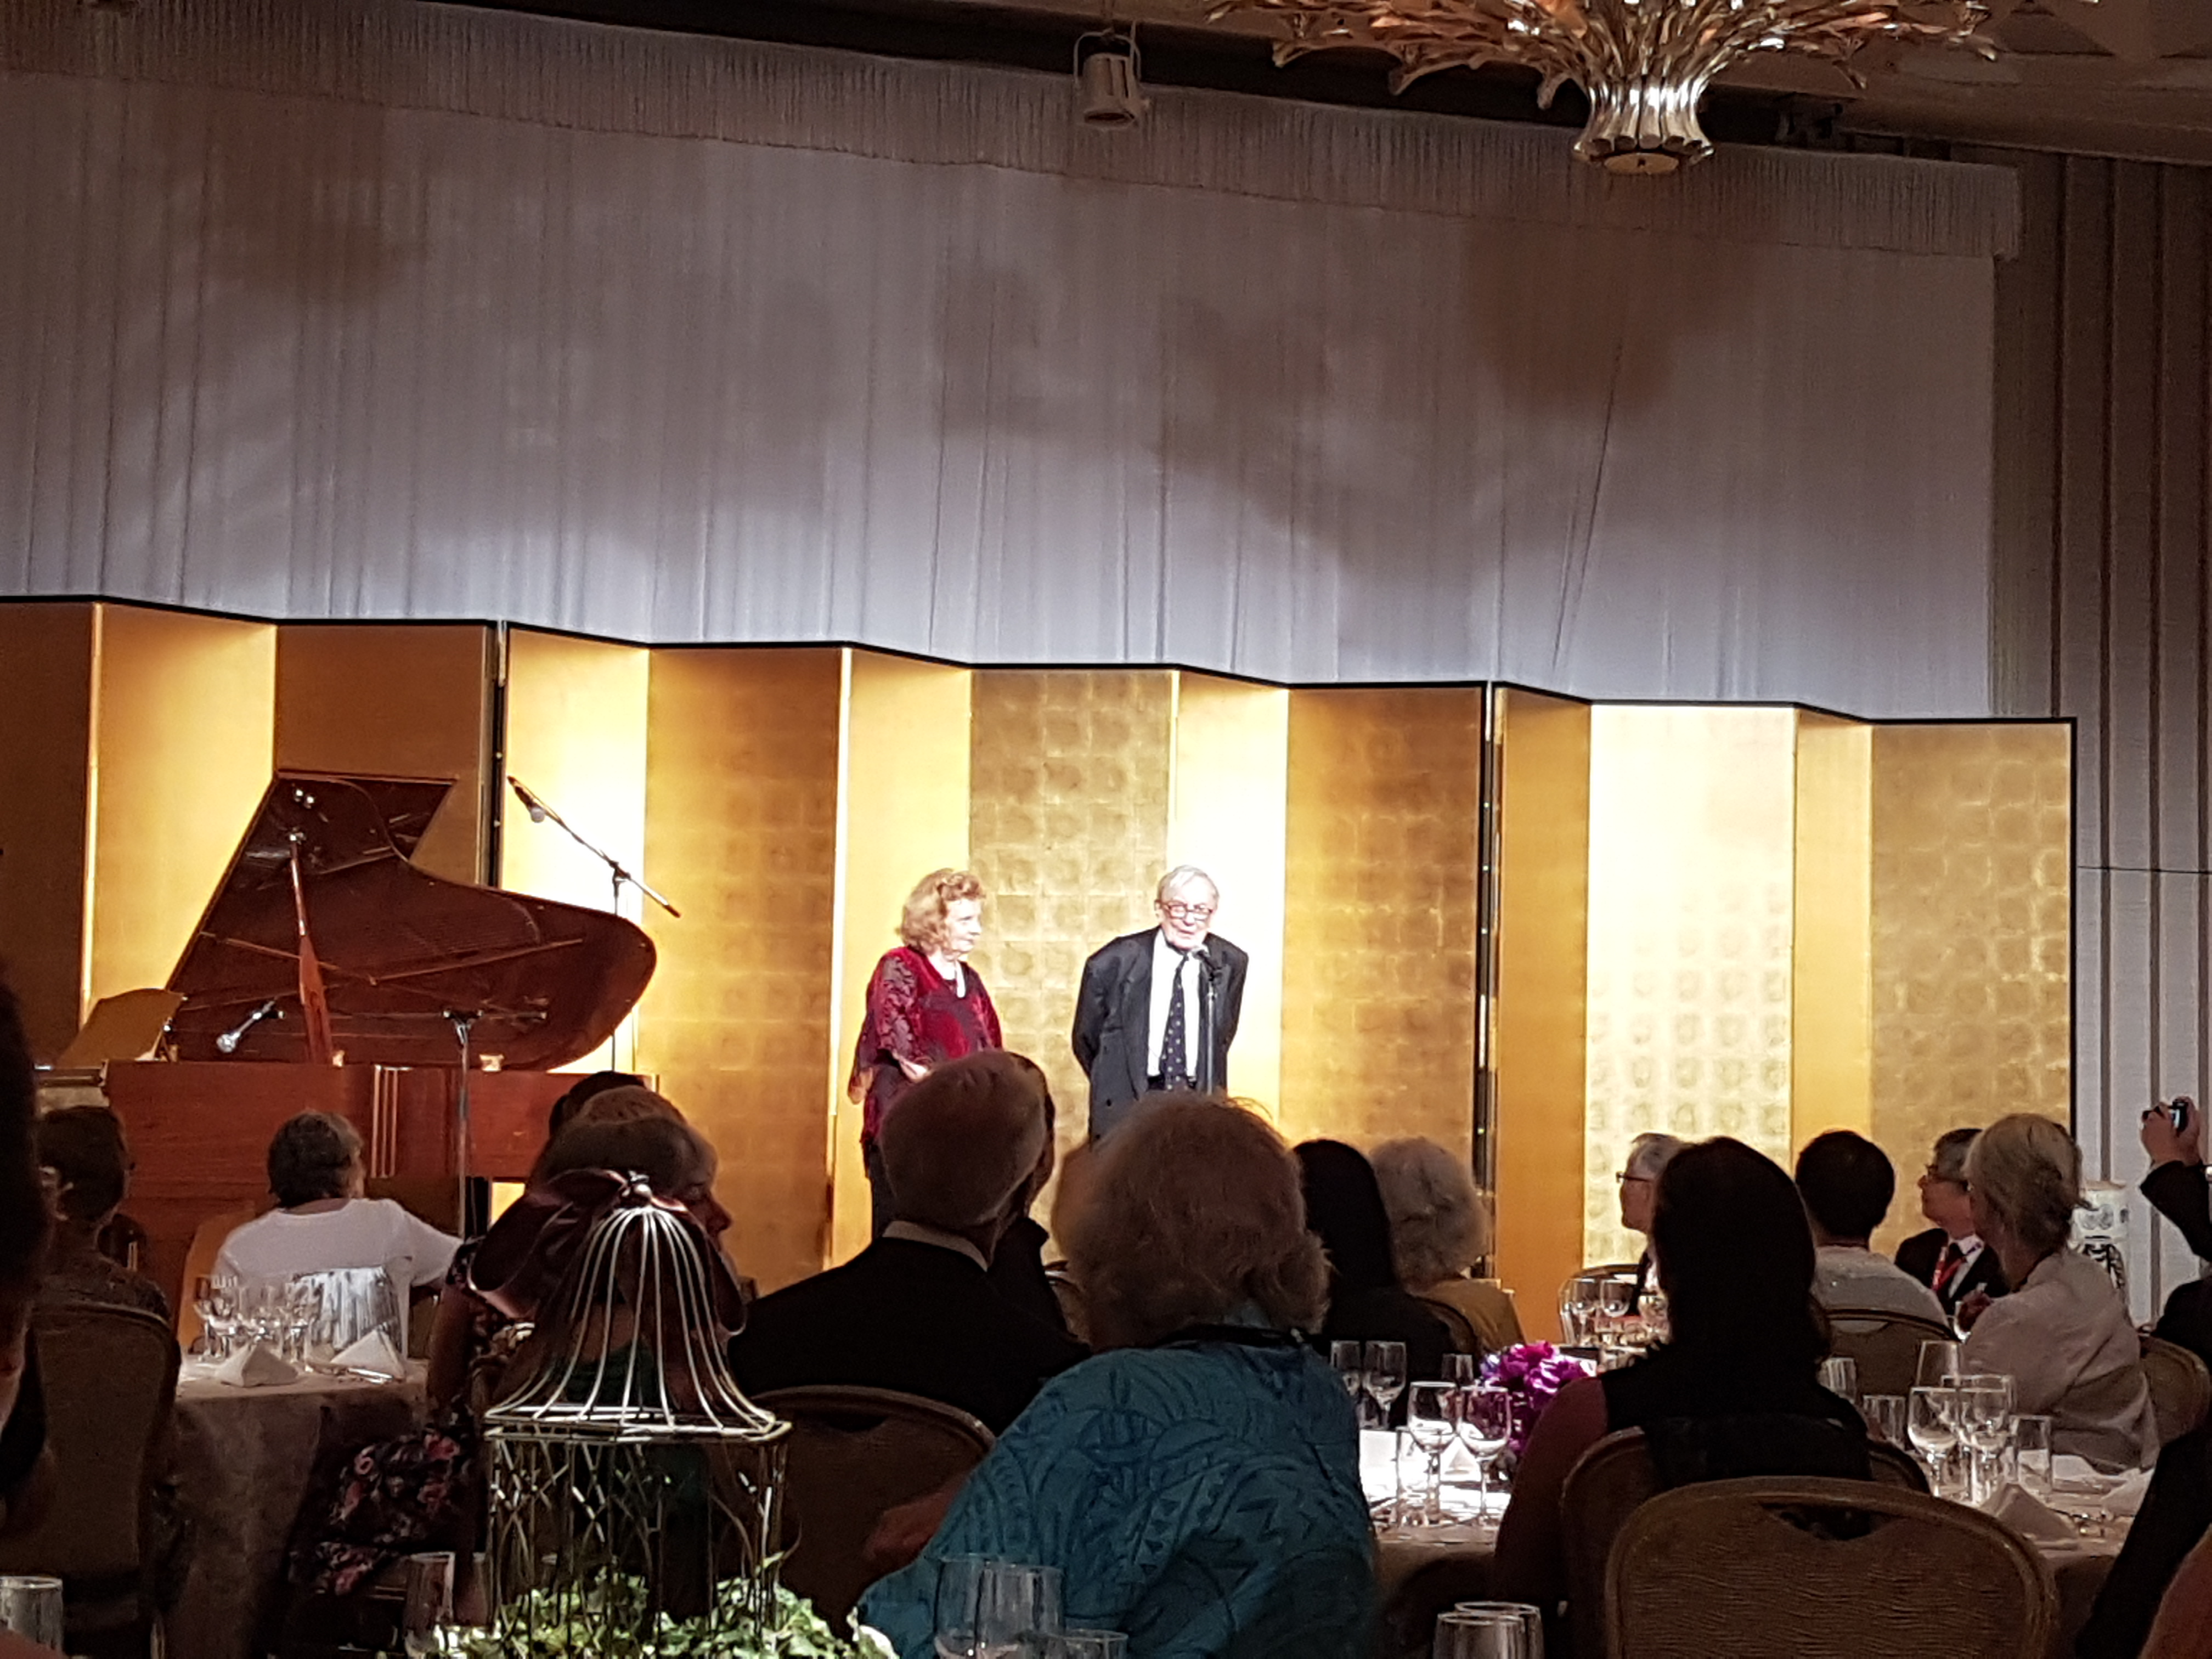
\includegraphics[width=\linewidth]{Hawkins-Figure06}
	\caption{Former President Claire Smith and Jack Golson at the Gala Dinner at Kyoto Brighton Hotel. 
		{\normalfont\scriptsize \\ \copyright\ by Antoinette Hennessy 2016}}
	\label{fig:Hawkins-Figure06}
\end{figure}

The closing day of the conference was a shorter half-day with fewer sessions and several events focusing on planning for WAC-9 in 2020. In particular, the vote for the host city for WAC-9 was cast.  Following the meeting of the WAC Assembly and the withdrawal of South Africa’s bid, it was voted that WAC-9 would be held in Prague, Czech Republic, in 2020. This will be the first WAC to be held in Eastern Europe. The detailed bid promised free public transport for all delegates and an opportunity to explore the vibrant and historic city of Prague. 

The closing ceremony \IJSRAsection{Closing ceremony}of WAC-8 was a poignant event, with the organisers taking the opportunity to honour the late Professor Joan Gero. Professor Gero was a well-loved member of the archaeological community who was heavily involved with WAC, tirelessly ensuring WAC’s future over many decades. The Vice-President of WAC, Anne Pyburn, and President Mizoguchi delivered the final address, and announced the creation of the Joan Gero Book Award in memory of Professor Gero. In her address, Anne Pyrburn reminded the audience of ongoing issues of racism, inequality, sexism and poverty in the world, and how the code of ethics upheld by WAC seeks to turn the tide on such attitudes. She noted that while great leaps had been taken in the last 30 years towards eradicating these issues, there was still a long way to go. 

Professor Pyburn used Professor Gero’s most recent publication, \textit{Yutopian} (2015), as an analogy for Professor Gero’s personal, professional and academic approach to the world and how she upheld the values of WAC in all aspects of her life. Professor Pyrburn stated: “Woven into the fabric of her science are all things WAC.” Professor Pyrburn described Yutopian as having “…set a standard of excellence to which we might aspire… As a realisation of WAC values it can serve the purpose of bequeathing WAC heritage to the next generation of members” \parencite{closingWAC}. To honour Joan and this pivotal publication, Professor Pyrburn announced this award would go to books best embodying WAC values, to be awarded every four years. The award has been endowed with travel money so that receiver might receive the award in person, beginning in 2020 at WAC 9 in Prague, Czech Republic. 

In closing, President Mizoguchi referenced his remarks at the Opening Ceremony, in particular his hope that WAC-8 would prove to be an ‘ideal speech situation’. Now at the end of the conference, President Mizoguchi stated that he had felt as though he was “in a dream” at WAC-8 because of how successfully this ‘ideal speech situation’ had eventuated \parencite{closingWAC}. However, he did remind us that in going back to our own individual communities we all have a responsibility to continue this conversation. 

The final event of WAC-8, the Farewell Party was also held at the Brighton Hotel, only a short distance from Doshisha University. Dr Mizoguchi delivered some final remarks, thanking the organising committee, volunteers and all participants before officially closing WAC-8 for 2016. 

\IJSRAseparator

Overall, WAC-8 \IJSRAsection{Comments}Kyoto was a pleasure to attend due to its inclusive atmosphere which, as students, was a welcomed feeling. The hope of achieving an ‘ideal speech situation’ as outlined by President Koji Mizoguchi in his opening address, was well and truly achieved with sessions and plenaries that sought to, and succeeded in, providing opportunities for debate, conversation and resolution. 

While the number of sessions on at any one time did prove challenging to navigate, the sheer number of topics covered throughout the sessions is a credit to the organisers and presenters, and a strong indicator of the WAC dedication to inclusivity.  It is important to acknowledge the number of presenters, including student presenters, with English as a second language; these presenters faced barriers those with English as their first language do not have to consider. President Mizoguchi described the language barrier as being one of the most difficult challenges that the organising committee faced. However, the success of the conference, the dedication of the WAC-8 volunteer force and the number of presenters with English as a second language indicates the success to which this barrier was overcome by all those involved. In a Facebook post thanking those who attended and organised WAC-8, President Mizoguchi stated that over 1,600 peopled participated in the conference from 83 different countries. As students attending their first WAC it was inspiring to meet so many other student attendees and note the number of students, both undergraduate and postgraduate, presenting their own research. Such diversity and inclusivity speaks of the spirit of WAC in a true meeting of global archaeology. 


%\IJSRAsection{small headline}

%\IJSRAseparator


\IJSRAclosing
%\end{otherlanguage}
%\end{document}